\documentclass[conference,compsoc]{IEEEtran}
\ifCLASSOPTIONcompsoc
  \usepackage[nocompress]{cite}
\else
  \usepackage{cite}
\fi
\ifCLASSINFOpdf
\else
\fi

\usepackage{listings}

\usepackage{graphicx}
\graphicspath{ {images/} }

\begin{document}
\title{MemSan: Progress report}

\author{\IEEEauthorblockN{Hugo Genesse}
\IEEEauthorblockA{Computer Engineering\\
Polytechnique Montreal\\
Montreal, Quebec\\
hugo.genesse@polymtl.ca}}

\maketitle
\begin{abstract}
MemSan is a user-supplied data flow analyzer targeting memory-sensitize functions like strcpy that could lead to buffer overflow vulnerabilities.
\end{abstract}

\IEEEpeerreviewmaketitle



\section{Introduction}
% no \IEEEPARstart

The second part of the project was to build UML class diagrams from
 C++ source code. This proved more difficult as it will be explained
 in the next sections. 

\section{Methodology}

Clang's ASTRecursiveVisitor was still used for the part
 that builds our own AST. Some parts were added and some
 were removed. Python classes for the analysis part of the project
 were also implemented to ease the next steps as it was mostly an hardcoded
 logic for the first part of the project and couldn't scale more.
 The code is available on github at svieg/MemSan.

\subsection{Implementation}

 For the UML class diagrams, I didn't need
 the number of local variables, break statements, if statements
 and while statements. As those could come in handy in the next steps,
 they were kept in the code of MemSan as comments. Only one
 visit was added, the FieldDecl one. This one provides a visit
 for the class attributes. The type also needed to be extracted
 in our AST. Luckily, the getType() method was defined with the
 getAsString() method to convert from internal clang types to strings.
 This was used for CXXRecordDecl which are classes and FieldDecl.
 For methods, getResultType() was called to resolve the return value type.
 This one proved tricky as it will be explained in the difficulties section later.
 For the XML part, the following tags were added: parentClass that stores the
 name of the base class in case the class MemSan is analyzing inherits from another one,
 methodReturnType that stores the return value type of that method. Also, since the
 attributes were new in this part of the project, I needed tags to identify them.
 We added the attribute tag to encapsulate all the attributes information
 As I couldn't get a real project meeting the course requirements to compile using my
 tool, the test called LOG6302\_TP1\_example.cpp was heavily modified to test the new use
 cases. I now use a base class named BaseClass that has one public and one private
 attribute and a method that returns a void*. One class inherits from this base class
 and is called ChildClass. The third and final class doesn't use inheritance but
 has an attribute that is of the type BaseClass. This example can then demonstrate
 most of the use cases.


\section{Results and Discussion}

Sadly, I couldn't get a real project to work on and had to work on a fake example
 that I created myself as discussed above.

\subsection{Results}

The UML class diagram that was created with MemSan is included in the appendix.


\subsection{Difficulties}

\subsubsection{Compilation}
Unfortunately, a lot of time was still spent trying to compile a real C++ project.
 My first project's choice was KVM but I realized that most of it is plain C and
 therefore doesn't the course requirements. I then tried several projects including
 chromium-os, firefox and chromium but all failed with my tests.

\subsubsection{Documentation}

Furthermore, I was using the public version of the documentation hosted on clang's
 website but used the 3.3 version while coding. Some features were lacking and
 it took me some time to realise why that was so.

\section{Conclusion}

I was able to create a UML class diagram from C++ source code but only in
 the example I created myself.



% use section* for acknowledgment
\ifCLASSOPTIONcompsoc
  % The Computer Society usually uses the plural form
  \section*{Acknowledgments}
    Nicolas Cloutier, best teaching assistant.
\else
  % regular IEEE prefers the singular form
  \section*{Acknowledgment}
\fi

\section{Appendix}

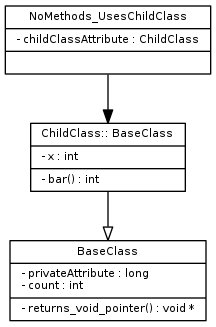
\includegraphics{graph}

\end{document}


